\chapter{Um Novo Protocolo Para Identidade Fiduciária}\label{ch:protocol}

O novo Protocolo para Identidade Fiduciária propõe uma modificação no protocolo \acs{OIDC4VP}, parte integrante do ecossistema \acs{OIDC4VC}, para adequá-lo ao Modelo Fiduciário. 
Através dessa adaptação facilitará a construção de uma camada de apresentação de credenciais de maneira simplificada, segura e amigável para os desenvolvedores. Destaca-se também a capacidade de reutilizar a infraestrutura existente, além do fácil acesso a uma vasta gama de códigos e bibliotecas desenvolvidas com base na especificação central do OpenID, o que amplifica sua adoção e integração. Essas características tornam o protocolo não apenas uma solução técnica eficiente, mas também uma abordagem estratégica que potencializa a escalabilidade e a interoperabilidade dentro do ecossistema de identidades digitais.

% % Pilha de protocolos 

% Além disso, a nova especificação introduz duas extensões que se alinham com as estratégias delineadas em \autoref{subsection:fiduciário} para a preservação da privacidade dos usuários: a Negociação de Atributos e a Negociação do Ambiente de Execução. A primeira utiliza a estrutura de \acs{DA}s em conjunto com a definição de novas mensagens e endpoints, visando à redução do risco de uso indevido de dados, garantindo que somente as informações estritamente necessárias sejam compartilhadas. De maneira similar, a segunda extensão, também baseada em  endpoints e mensagens, possibilita que dados e informações sensíveis sejam preferencialmente processados em ambientes confiáveis para o usuário. Essas inovações visam não apenas cumprir os requisitos de segurança, mas também aprimorar a confiança do usuário no sistema, ao assegurar que sua privacidade seja rigorosamente protegida em todas as etapas do processo.

% Dessa forma, este texto busca detalhar as adaptações requeridas no \acs{OIDC4VP} para garantir sua conformidade com a pilha especificada na \autoref{fig:stack-model-protocol-extension}, onde os protocolos e extensões são integrados para satisfazer as propriedades e comportamentos preconizados pelo Modelo Fiduciário. Essas adaptações asseguram o alinhamento com os princípios de privacidade estabelecidos por regulamentações como a \sigla{LGPD}{Lei Geral de Proteção de Dados}, representando um avanço significativo na evolução das identidades digitais, promovendo uma solução que equilibra inovação tecnológica com os mais altos padrões de proteção de dados.

% Assim, este texto tem como objetivo detalhar as adaptações necessárias no OIDC4VP para garantir sua conformidade com a pilha especificada na Figura 13. Essa pilha ilustra uma abordagem modular que pode ser utilizada para alcançar as propriedades e comportamentos previstos pelo Modelo Fiduciário. Embora o foco principal esteja na adaptação do \acs{OIDC4VP}, destacado em tons de cinza, deixa em aberto a viabilidade de explorar as demais soluções mencionadas em \autoref{subsec:oidc4vc}, representadas em branco, e adaptá-las para atender aos demais princípios previstos no modelo.

A nova especificação introduz duas extensões alinhadas às estratégias da \autoref{subsection:fiduciário} para a preservação da privacidade dos usuários: a \emph{Negociação de Atributos} e a \emph{Negociação do Ambiente de Execução}. A primeira utiliza a estrutura de \acs{DA}s em conjunto com a definição de novas mensagens e endpoints, visando à redução do risco de uso indevido de dados, garantindo que somente as informações estritamente necessárias sejam compartilhadas. Já a segunda extensão, também baseada em endpoints e mensagens, permite que dados sensíveis sejam preferencialmente processados em ambientes confiáveis ao usuário.

Essas adaptações são representadas na \autoref{fig:stack-model-protocol-extension}, que adota uma abordagem modular como solução para atingir as propriedades e comportamentos definidos pelo modelo. Embora o foco esteja no \acs{OIDC4VP}, destacado em tons de cinza, deixa-se em aberto a viabilidade de explorar as demais soluções mencionadas em \autoref{subsection:fiduciário}, representadas em branco, para atender aos demais princípios do modelo.
Essa solução visa não apenas cumprir os requisitos de segurança, mas também aprimorar a confiança do usuário no sistema, ao assegurar que sua privacidade seja rigorosamente protegida em todas as etapas do processo.

\begin{figure}[htb]
    \caption{Pilha: Modelo, protocolos, extensões.}
    \centering
    \resizebox{\linewidth}{!}{
        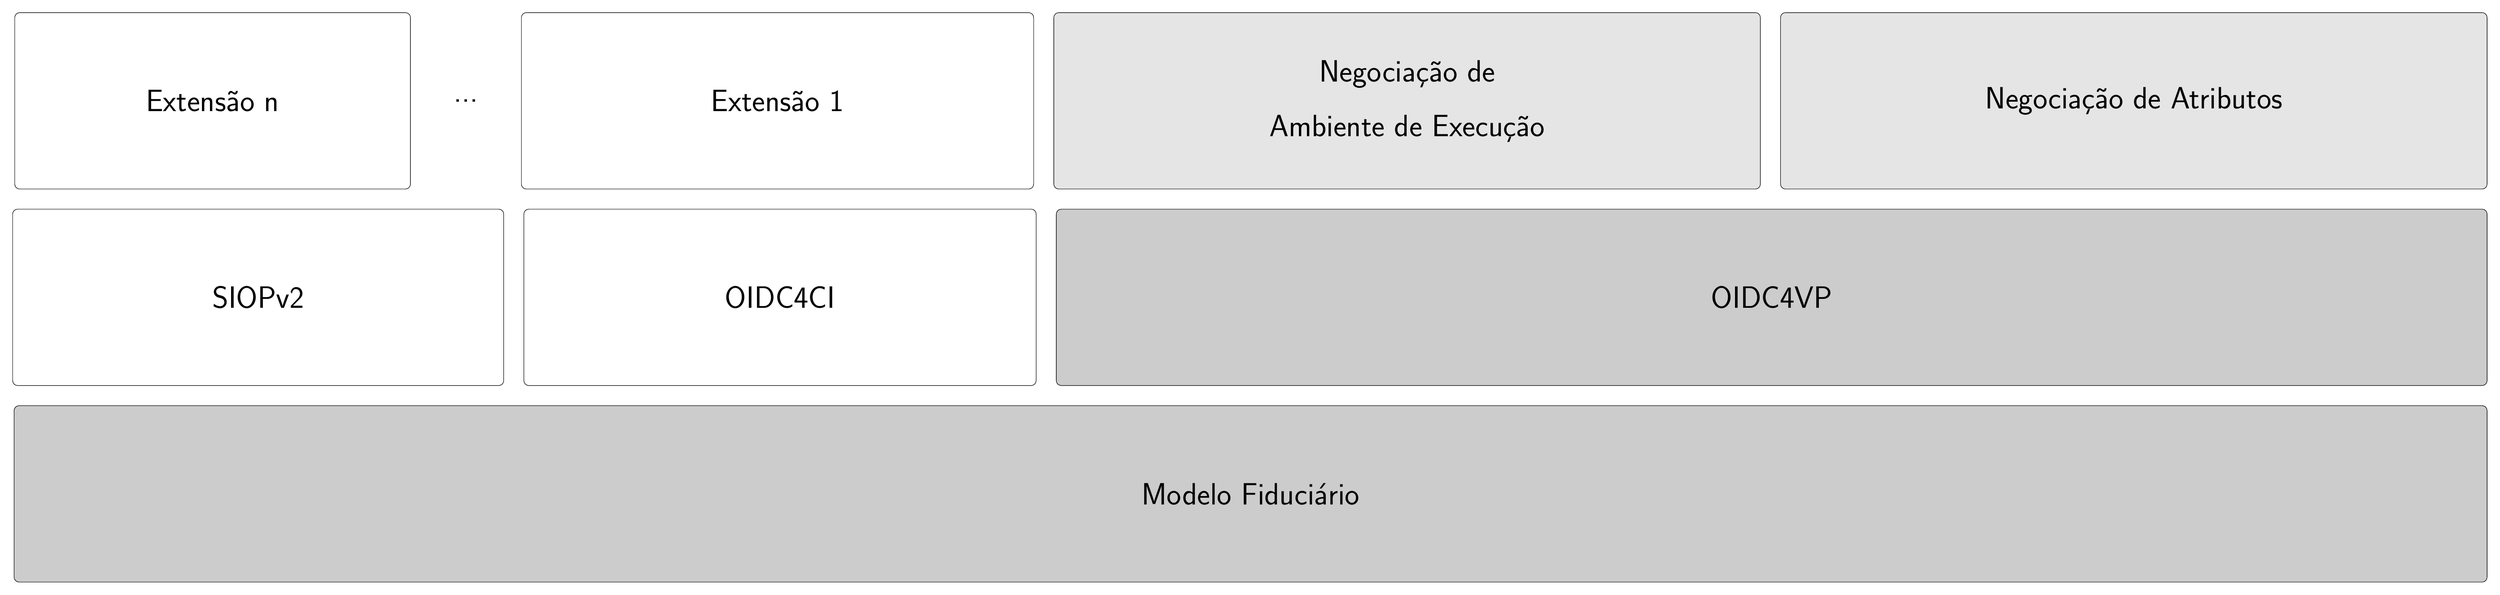
\begin{tikzpicture}[node distance=1cm,outer sep=1pt,inner sep=1pt]

    % CONFIGURANDO OS NODOS 
 
    %------------------------ CAMADA 3----------------------------%
    \tikzset{field/.style={align=center,shape=rectangle,rounded corners,minimum height=5cm,minimum width=20cm,draw,font=\fontsize{36}{44}\selectfont\sffamily,fill=gray!20}}

    \tikzset{field2/.style={align=center,shape=rectangle,rounded corners,minimum height=5cm,minimum width=29cm,draw,font=\fontsize{36}{44}\selectfont\sffamily,fill=gray!20}}

    %------------------------ CAMADA 2----------------------------%
    \tikzset{mediumfield/.style={align=center,shape=rectangle,rounded corners,minimum height=5cm,minimum width=40.5cm,draw,font=\fontsize{36}{44}\selectfont\sffamily,fill=gray!40}}

    \tikzset{mediumfield2/.style={align=center,shape=rectangle,rounded corners,minimum height=5cm,minimum width=14.5cm,draw,font=\fontsize{36}{44}\selectfont\sffamily,fill=gray!40}}

    \tikzset{mediumfield3/.style={align=center,shape=rectangle,rounded corners,minimum height=5cm,minimum width=13.9cm,draw,font=\fontsize{36}{44}\selectfont\sffamily,fill=gray!40}}

 %------------------------ CAMADA 1----------------------------%
    \tikzset{largefield/.style={align=center,shape=rectangle,rounded corners,minimum height=5cm,minimum width=70cm,draw,font=\fontsize{36}{44}\selectfont\sffamily,fill=gray!40}}


    % INSTANCIANDO OS NODOS
    
    %------------------------ CAMADA 1----------------------------%
    % Desenho do primeiro retângulo (grande)
    \node [largefield] (fid) {Modelo Fiduciário};


    %------------------------ CAMADA 2----------------------------%
    % Desenho do segundo retângulo (médio), alinhado à direita com o primeiro, e posicionado acima
    \node [mediumfield,anchor=south east] at ([yshift=0.5cm]fid.north east) (oidc4vp) {OIDC4VP};

     % Desenho do segundo retângulo (médio), alinhado à direita com o primeiro, e posicionado acima
    \node [mediumfield2,anchor=south east, fill=white] at ([xshift=-0.5cm]oidc4vp.south west) (oidc4ci) {OIDC4CI};

    \node [mediumfield3,anchor=south east, fill=white] at ([xshift=-0.5cm]oidc4ci.south west) (siopv2) {SIOPv2};
    %------------------------ CAMADA 3----------------------------%

    \node [field,anchor=south east] at ([yshift=0.5cm]oidc4vp.north east) (atributes) {Negociação de Atributos};
    
    \node [field,anchor=south east] at ([xshift=-0.5cm]atributes.south west) (env) {Negociação de \\ Ambiente de Execução};

    % \node [mediumfield2,anchor=south east, fill=white, minimum width=14cm] at ([xshift=-0.5cm]env.south west) (ext1) {Extensão 1};
    \node [mediumfield2,anchor=south east, fill=white, minimum width=14.5cm] at ([xshift=-0.5cm]env.south west)  (ext1) {Extensão 1};
    \node [mediumfield2,anchor=south east, fill=white, minimum width=2cm, draw=white] at ([xshift=-0.5cm]ext1.south west) (dots) {...};
    \node [mediumfield2,anchor=south east, fill=white, minimum width=11.2cm] at ([xshift=-0.5cm]dots.south west) (extn) {Extensão n};    

    % \node [mediumfield2,anchor=south east, fill=white, draw=white] at ([xshift=-0.5cm]ext1.south west) (env) {\large{...}};
    % \node [field2,anchor=south east] at ([xshift=-0.5cm]env.south west) (aud) {Auditoria};
    
    
    
\end{tikzpicture}
    }
    \fonte{O Autor}
    \label{fig:stack-model-protocol-extension}
\end{figure}

\section{Integração do OIDC4VP com o Modelo Fiduciário}

A transição do modelo original de \acs{SSI}, no qual o \acs{OIDC4VP} foi originalmente proposto, para o Modelo Fiduciário, é um processo bastante natural como mostrado na \autoref{fig:oidc4vp-in-fid}. 
Isso ocorre porque esta adaptação foca exclusivamente na redução da divulgação de dados proposto por \emph{Non-Disclousure as Goal}, sem exigir, por exemplo, modificações nas mensagens trocadas pelo Fiduciário como solução para garantir maior controle sobre as ações realizadas com os dados do usuário, conforme previsto no princípio de \emph{Transparency for Accountability}.
Dessa forma, não foram necessárias alterações significativas, permitindo que a \acs{SP} continue desempenhando seu papel como a entidade responsável por solicitar, receber e validar as \acs{VP}s. No contexto do \acs{OIDC4VP}, essa função é exercida por meio do papel de Cliente OAuth.

O Fiduciário, por sua vez, possui as mesmas funções e capacidades que a Carteira, conforme discutido anteriormente na \autoref{subsection:fiduciário}, incluindo receber, armazenar, apresentar e gerenciar as \acs{VC}s, bem como as chaves criptográficas associadas. Portanto, no contexto do \acs{OIDC4VP}, deve assumir o papel Servidor de Autorização que é realizado pela Carteira dentro desse contexto. No entanto, com a prioridade de, além de adquirir um mecanismo para entregar \acs{VP}s, integrar as extensões de \emph{Negociação de Atributos} e \emph{Negociação do Ambiente de Execução} nos fluxos existentes, visando atender o pilar \emph{Non-Disclosure as Goal}.
% Mudanças em oidc4vp
\begin{figure}[htb]
    \caption{Fluxo com Fiduciário no lugar da Carteira}
    \centering
    \resizebox{\linewidth}{!}{\begin{sequencediagram}[scale=0.1]
    \newthread{A}{\ttfamily Usuário}{}
    \newinst[4]{C}{\ttfamily Fiduciário}{}
    \newinst[11]{B}{\ttfamily \acs{SP}}{}
    
    \newcounter{number}
    \stepcounter{number}
    \begin{call}{A}{\ttfamily Interação}{B}
        \postlevel
        \postlevel
        \postlevel
        \stepcounter{number}
            \begin{call}{B}{\shortstack{ \ttfamily (1) Requisição de Autorização \\ \ttfamily (client\_id, nonce, redirect\_uri, presentation\_definition)}}{C}{\shortstack{\ttfamily (2) Resposta de Autorização \\ \ttfamily (vp\_token, presenation\_submission)}}
            \postlevel
            \postlevel

            % Adicionando uma nota após o passo 1
            \node at (1.5,-4) [text width=6cm, anchor=west] {\ttfamily \small Autenticação e Confirmação/Seleção da \acs{VC}};

            \postlevel
            
        \end{call}
    \end{call}
\end{sequencediagram}}
    
    \label{fig:oidc4vp-in-fid}
    \fonte{O Autor}
\end{figure}

\section{Uso de Provas de Conhecimento Zero}

A utilização da especificação OIDC4VP no Modelo Fiduciário visa aproveitar a flexibilidade e a concepção agnóstica em relação ao formato das Credenciais Verificáveis utilizadas. Isso significa que sua adaptação ao modelo não exige diretamente o uso de Provas de Conhecimento Zero; ao contrário, proporciona um ambiente que permite a integração de \acs{VC}s que possuam essa capacidade. Como o \acs{OIDC4VP} não estabelece requisitos específicos para a implementação de \acs{ZKP}, cabe aos formatos de \acs{VC}s adotados determinar se oferecem suporte ou não para essa tecnologia. O uso dessa tecnologia é recomendado especialmente em contextos que exigem altos níveis de privacidade e segurança na verificação das credenciais, permitindo que apenas as informações estritamente necessárias sejam divulgadas.

\section{Negociação de Atributos}\label{section:attribute-negotiation}

Quando um Fiduciário recebe uma Requisição de Autorização é possível que a Definição de Apresentação solicite informações do usuário as quais não estejam de acordo com as Políticas de Consentimento definidas previamente. Por exemplo, é comum que Provedores de Serviço realizem a solicitação da data de nascimento dos  usuários apenas para verificar sua maioridade. Este tipo de requisição é invasiva e pode estar contra os desejos do indivíduo. Dessa forma, a extensão \textbf{Negociação de Atributos} permite definir quais informações sobre os usuários são relevantes para a plataforma que está oferecendo serviços sem comprometer a privacidade e o sigilo dos dados do dono desses recursos.

Esse mecanismo está centrado na estrutura de \acs{DA}s, que no modelo Fiduciário são chamados de \textbf{Declarações de Requisitos} (Requirements Statements). Neste texto, os termos \acs{DA}s e Declarações de Requisitos serão tratados como sinônimos. Com essa estrutura, os Fiduciários conseguem definir quais informações requisitadas não estão em conformidade com as Políticas de Consentimento e propor novos que satisfaçam as intenções. Para que isso seja possível, são definidos o endpoint Negociação (Negotiation Endpoint), a Solicitação de Negociação (Negotiation Request) e sua respectiva resposta, Resposta de Negociação (Negotiation Response). 
Essa nova requisição, iniciada pelo Fiduciário e respondida pelo \acs{SP}, ocorre entre a Requisição de Autorização e sua respectiva resposta, conforme destacado na \autoref{fig:attribute-negotiation-flow-via-browser}.

\begin{figure}[htb]
    \caption{Fluxo para Negociação de Atributos.}
    \centering
    \resizebox{\linewidth}{!}{\begin{sequencediagram}[scale=0.1]
    \newthread{A}{\ttfamily Usuário}{}
    \newinst[6]{B}{\ttfamily Fiduciário}{}
    \newinst[15]{C}{\ttfamily \acs{SP}}{}
    
    \begin{call}{A}{\ttfamily Interação}{C}
        \postlevel
        \postlevel
        \postlevel
            \begin{call}{C}{\shortstack{ \ttfamily (1) Requisição de Autorização \\ \ttfamily (client\_id, nonce, redirect\_uri, presentation\_definition, client\_metadata)}}{A}{\shortstack{\ttfamily (2) Resposta de Autorização \\ \ttfamily (vp\_token, presenation\_submission)}}
            \postlevel
            \postlevel

            \begin{call}{A}{\shortstack{ \ttfamily (1) Requisição de Autorização}}{B}{\shortstack{\ttfamily (2) Resposta de Autorização}}

                \postlevel
                \postlevel
                % Adicionando uma nota após o passo 1
                % \node at (1.5,-4) [text width=6cm, anchor=west] {\ttfamily \small Autenticação e Confirmação/Seleção da \acs{VC}};
    
                \postlevel
                \begin{call}{B}{\shortstack{  \bfseries\ttfamily Requisição de Negociação \\ \bfseries\ttfamily (type, definition\_id, presentation\_definition)}}{C}{\shortstack{ \ttfamily \bfseries Resposta de Negociação\\ \bfseries\ttfamily(status)}}
                \postlevel
                \end{call}

            \postlevel  
            \end{call}

            \postlevel
            \postlevel
            
        \end{call}
    \end{call}
\end{sequencediagram}

}
    \fonte{O Autor}
    \label{fig:attribute-negotiation-flow-via-browser}
\end{figure}


\subsection{Endpoint de Negociação}\label{subsection:endpoint-negociação}

Este endpoint é utilizado para negociar Declaração de Requisitos previamente encaminhada em casos os quais o Fiduciário identifica alguma divergência do que foi requisitado e o que é autorizado dentro das Políticas de Consentimento. A comunicação com o Endpoint de Neogicação deve utilizar TLS.

Para o Fiduciário obter o \emph{Endpoint de Negociação} do Provedor de Serviços, este texto define o parâmetro \texttt{negotiation\_endpoint}, que pode ser adquirido por dois meios. O primeiro é pelo mecanismo tradicional de registro \acs{OIDC-D} de \cite{sakimura2023openidDiscovery}, no qual os Clientes OAuth fornecem seus metadados aos Servidores de Autorização. O segundo é por meio do parâmetro \texttt{client\_metadata}, conforme definido na seção 5 \cite{OIDC4VP2023}, enviado na Requisição de Autorização e contendo os metadados do \acs{SP}.

\begin{itemize}
    \item \textbf{negotiation\_endpoint}: URL do Endpoint de Negociação do Provedor de Serviços. Esta URL deve usar o esquema HTTPS e pode conter componentes de porta, caminho e parâmetros de consulta. Se omitido, o provedor não oferece suporte a esse endpoint e não está em conformidade com as propriedades do Modelo Fiduciário.
\end{itemize}

% Endpoint de Negocição
\begin{figure}[htb]
    \caption{Exemplo de parâmetro negotiation\_enpoint no client\_metadata (em UTF-8).}
    \centering
    \input{code/json}


% Exemplo baseado na Seção 5 (Authorization Request) do OIDC4VP
\begin{lstlisting}[language=json,firstnumber=1]
GET /authorize?
  client_id=client.example.org
  &client_metadata=%7B%22vp_formats%22%3A%7B%22jwt_vp_json%22%3A%7B%22alg%22%3A%5B%22EdDSA%22%2C%22ES256K%22%5D%7D%7D%2C%22negotiation_endpoint%22%3A%22https%3A%2F%2Fexample.com%22%7D
  &request_uri=https%3A%2F%2Fclient.example.org%2Frequest%2Fvapof4ql2i7m41m68uep
  &request_uri_method=post HTTP/1.1
\end{lstlisting}
    \fonte{O Autor}
    \label{fig:negotiation-endpoint}
\end{figure}

\subsection{Solicitação de Negociação}\label{subsection:negotiation-request}

A Solicitação de Negociação constitui uma requisição HTTP POST enviada pelo Fiduciário ao \acs{SP}, com o tipo de mídia \texttt{application/json}. Os parâmetros utilizados na solicitação são os seguintes:

% Requisição de Negociação
\begin{figure}[htb]
    \caption{Solicitação de Negociação.}
    \centering
    \input{code/json}

\begin{lstlisting}[language=json,firstnumber=1]
POST /negotiate HTTP/1.1
Host: example.com
Content-Type: application/json

{
  "type": "attribute",
  "definition_id": "8xLOxBtZp8",
  "presentation_definition": "..."
}
\end{lstlisting}
    \fonte{O Autor}
    \label{fig:negotiation-request}
\end{figure}

\begin{itemize}

    \item \textbf{type}: OBRIGATÓRIO. Este parâmetro deve ser utilizado na Solicitação de Negociação para especificar o tipo de negociação que está sendo realizada. No contexto da \emph{Negociação de Atributos}, deve-se utilizar o valor \texttt{attribute}.

    \item \textbf{definition\_id}: OPCIONAL. Trata-se de uma string que identifica uma Declaração de Requisitos previamente encaminhada ao Fiduciário. Após o acordo ser firmado entre o Fiduciário e o Provedor, o \acs{SP} deve invalidar o \texttt{definition\_id}. Este parâmetro se torna OBRIGATÓRIO quando o valor de \texttt{type} é \texttt{attribute}.
    
    \item \textbf{presentation\_definition}: OPCIONAL. Este parâmetro contém um objeto JSON de Declaração de Requisitos, conforme a sintaxe estabelecida na \cite{presentation-exchange}. Este parâmetro se torna OBRIGATÓRIO quando o valor de \texttt{type} é \texttt{attribute}.
    
\end{itemize}

\subsection{Resposta de Negociação}

O Provedor de Serviços possui a prerrogativa de aceitar ou recusar a proposta de alteração da Declaração de Requisitos. Em determinados casos, o Fiduciário aceita a proposta que contém a nova Declaração de Requisitos e responde com uma mensagem com tipo de mídia \texttt{application/json} contendo em seu corpo o \acs{JSON} com o parâmetro status indicando a aceitação da sugestão de declaração e o código de status HTTP 202 sinalizando está pronto para receber a nova declaração, que é diferente daquele que o \acs{SP} enviou em sua Requsição de Autorização. 

% % Resposta de Negocição bem sucedida
\begin{figure}[htb]
    \caption{Resposta de Negociação com Sucesso}
    \centering
    \input{code/json}

\begin{lstlisting}[language=json,firstnumber=1]
HTTP/1.1 202 Accepted
Content-Type: application/json

{
    "status": "accepted",
}

\end{lstlisting}
    \fonte{O Autor}
    \label{fig:negotiation-response-success}
\end{figure}

\begin{itemize}
    
   \item \textbf{status}: OBRIGATÓRIO. A semântica desse campo irá depender da negociação definida em type. Nesse exemplo, indica se o \acs{SP} aceitou ou recusou a nova proposta para a Declaração de Requisitos. O código de status em formato ASCII selecionado entre as duas opções abaixo:

    \begin{itemize}
        \item \textbf{accepted}: Indica que a proposta para a nova Declaração de Requisitos foi aceita pelo \acs{SP}. Nesse caso, o processo de alteração da Declaração de Requisitos será iniciado, e o recurso associado pode ser atualizado ou criado conforme necessário.
        
        \item \textbf{refused}: Indica que a proposta para a nova Declaração de Requisitos foi recusada pelo \acs{SP}. Nesse caso, nenhuma alteração será realizada, e a Declaração de Requisitos permanecerá como está. O motivo da recusa pode ser detalhado em um campo adicional de erro chamado \texttt{error\_description}, descrito a seguir.
    \end{itemize}

\end{itemize}

Em outros casos, o \acs{SP} pode rejeitar a proposta por não concordar com os novos sugeridos. Nessas situações, a resposta HTTP deve utilizar o parâmetro status rejeitando a declaração e o código de status HTTP 400 (Bad Request) incluindo os seguintes parâmetros no corpo da resposta codificada em JSON.

\subsubsection*{Resposta de Recusa de Negociação}\label{subsubsection:response-negotiation-error}

Se a Solicitação de Negociação não for aceita por não atender aos requisitos da aplicação, ou for considerada inválida devido à sintaxe incorreta da requisição, o SP deverá definir o campo de status como \texttt{refused} e incluir os campos \texttt{error} e \texttt{retry\_after}, conforme ilustrado abaixo.

% % Resposta de Negocição com falha
\begin{figure}[htb]
    \caption{Resposta de Negociação com Recusa}
    \centering
    \input{code/json}

\begin{lstlisting}[language=json,firstnumber=1]
HTTP/1.1 400 Bad Request
Content-Type: application/json

{
    "status": "refused",
    "error": "invalid_negotiation_request",
    "retry_after": 10
}

\end{lstlisting}
    \fonte{O Autor}
    \label{fig:negotiation-response-refused}
\end{figure}

\begin{itemize}

    \item \textbf{Error}: OBRIGATÓRIO. O parâmetro de erro deve conter um único código de erro em formato ASCII selecionado a partir da lista a seguir:

    \begin{itemize}
    
        \item \textbf{negotiation\_request\_denied}: A semântica desse campo irá depender da negociação definida em type. Nesse contexto, indica que a Solicitação de Negociação com a nova Declaração de Requisitos não foi aceita pelo provedor de serviços.

        \item \textbf{invalid\_negotiation\_request}: A Solicitação de Negociação está incompleta, com falta de um parâmetro obrigatório, inclui um parâmetro ou valor de parâmetro não suportado, repete o mesmo parâmetro ou está de outra forma malformada.

        \item \textbf{unsupported\_definition}: A Declaração de Requisitos contida na Solicitação de Negociação contém um formato que não é reconhecido ou suportado pelo \acs{SP}. Esse erro acontece quando é utilizada uma versão desatualizada ou por não seguir a sintaxe e os padrões estabelecidos.

        \item \textbf{expired\_definition\_id}: Esse erro indica que o \texttt{definition\_id} fornecido na Solicitação de Negociação já expirou. Isso ocorre quando a negociação associada a esse \texttt{definition\_id} já foi concluída e o identificador pode ser invalidado para impedir que novas solicitações sejam feitas com base em um estado anterior.
        
    \end{itemize}

    \item \textbf{error\_description}: OPCIONAL. O parâmetro \texttt{error\_description} deve ser um texto ASCII, fornecendo informações adicionais para ajudar os implementadores do Fiduciário a entender o erro ocorrido. Ele pode incluir espaços, caracteres de pontuação e símbolos comuns, mas não pode incluir caracteres como o caractere aspas duplas ("), barra invertida (\textbackslash), ou qualquer caractere de controle esteja fora dos intervalos \texttt{\%x20-21 / \%x23-5B / \%x5D-7E}, onde o prefixo \texttt{\%} indica valores hexadecimais da tabela ASCII.

    \item \textbf{retry\_after}: OBRIGATÓRIO. A resposta de erro deve também conter o parâmetro \texttt{retry\_after}, que determina o tempo mínimo em segundos que o Fiduciário deve aguardar antes de enviar uma nova solicitação ao Endpoint de Negociação.
    
\end{itemize}


Se o Fiduciário e o Provedor de Serviços não chegarem a um acordo sobre a Declaração de Requisitos, ambos continuarão a trocar mensagens até atingirem um limite estipulado por uma das partes. Assim, recomenda-se fortemente que o Provedor de Serviços adote práticas flexíveis, solicitando apenas as informações estritamente necessárias. Caso contrário, a ausência de um acordo pode resultar na perda de acesso ao serviço pelo usuário, o que pode afetar negativamente a percepção pública da marca, gerando comentários desfavoráveis e reclamações que podem se espalhar rapidamente.

% \begin{figure}[htb]
    \caption{Fluxo para Negociação de Atributos}
    \centering
    \resizebox{\linewidth}{!}{\begin{sequencediagram}[scale=0.1]
    \newthread{A}{\ttfamily Usuário}{}
    \newinst[4]{B}{\ttfamily Fiduciário}{}
    \newinst[15]{C}{\ttfamily \acs{SP}}{}
    
    \begin{call}{A}{\ttfamily Interação}{C}
        \postlevel
        \postlevel
        \postlevel
            \begin{call}{C}{\shortstack{ \ttfamily (1) Requisição de Autorização \\ \ttfamily (client\_id, nonce, redirect\_uri, presentation\_definition, client\_metadata)}}{B}{\shortstack{\ttfamily (2) Resposta de Autorização \\ \ttfamily (vp\_token, presenation\_submission)}}
            \postlevel

            % Adicionando uma nota após o passo 1
            \node at (1.5,-4) [text width=6cm, anchor=west] {\ttfamily \small Autenticação e Confirmação/Seleção da \acs{VC}};

            \postlevel

            \begin{call}{B}{\shortstack{ \ttfamily Requisição de Negociação\\ \ttfamily (type, definition\_id, presentation\_definition)}}{C}{\shortstack{ \ttfamily Resposta de Negociação\\ \ttfamily(status)}}

            \postlevel
                
            \end{call}

            \postlevel
            \postlevel
            
        \end{call}
    \end{call}
\end{sequencediagram}

}
    \fonte{O Autor}
    \label{fig:attribute-negotiation-flow}
\end{figure}



\clearpage
\section{Negociação do Ambiente de Execução}\label{section:env-negotiation}

As arquiteturas tecnológicas vigentes, de modo geral, adotam a lógica de que a manipulação dos dados dos usuários deve ocorrer exclusivamente no lado do \acs{SP}, centralizando o processamento e o armazenamento das informações. No entanto, novas alternativas estão surgindo e possibilitam uma mudança nesse paradigma, como é o caso da proposta de execução dentro do Fiduciário, visto na \autoref{subsection:fiduciário}, e o uso de \acs{MPC}. Essas soluções permitem que o processamento de dados sensíveis seja realizado de forma descentralizada e segura, protegendo a privacidade do usuário ao restringir o acesso direto aos dados pelo provedor de serviços e permitindo que o processamento ocorra de maneira distribuída e controlada. 

Nesse sentido, a especificação de \textbf{Negociação do Ambiente de Execução} viabiliza esses dois paradigmas dentro do Modelo Fiduciário, possibilitando que o beneficiário decida o local (Fiduciário ou \acs{SP}) e forma (tradicional ou \acs{MPC}) apropriada para o processamento de suas informações privadas. O objetivo dessa mudança é manter o paradigma atual em operação, enquanto abre espaço para a integração dessas novas abordagens em serviços compatíveis. A especificação está centrada nas solicitações e endpoints mencionados na \autoref{subsection:negotiation-request} e possibilita o usuário decidir em qual local é o melhor para que suas informações sejam processadas, conforme pode ser visto na \autoref{fig:env-negotiation-flow}.

\begin{figure}[htb]
    \caption{Fluxo para Negociação de Ambiente de Execução.}
    \centering
    \resizebox{\linewidth}{!}{% \begin{sequencediagram}[scale=0.1]
%     \newthread{A}{\ttfamily Usuário}{}
%     \newinst[4]{C}{\ttfamily Fiduciário}{}
%     \newinst[18]{B}{\ttfamily \acs{SP}}{}
    
%     \begin{call}{A}{\ttfamily Interação}{B}
%         \postlevel
%         \postlevel
%         \postlevel
%             \begin{call}{B}{\shortstack{ \ttfamily (1) Requisição de Autorização \\ \ttfamily (client\_id, nonce, redirect\_uri, presentation\_definition, client\_metadata)}}{C}{\shortstack{\ttfamily (2) Resposta de Autorização \\ \ttfamily (vp\_token, presenation\_submission)}}
%             \postlevel

%             % Adicionando uma nota após o passo 1
%             \node at (1.5,-4) [text width=6cm, anchor=west] {\ttfamily \small Autenticação e Confirmação/Seleção da \acs{VC}};

%             \postlevel

%             \begin{call}{C}{\shortstack{ \ttfamily \bfseries Requisição de Negociação\\ \ttfamily \bfseries (type, compute\_site, compute\_site\_description)}}{B}{\shortstack{ \ttfamily \bfseries Resposta de Negociação\\ \bfseries \ttfamily(status)}}

%             \postlevel
                
%             \end{call}

%             \postlevel
%             \postlevel
            
%         \end{call}
%     \end{call}
% \end{sequencediagram}

\begin{sequencediagram}[scale=0.1]
    \newthread{A}{\ttfamily Usuário}{}
    \newinst[6]{B}{\ttfamily Fiduciário}{}
    \newinst[15]{C}{\ttfamily \acs{SP}}{}
    
    \begin{call}{A}{\ttfamily Interação}{C}
        \postlevel
        \postlevel
        \postlevel
            \begin{call}{C}{\shortstack{ \ttfamily (1) Requisição de Autorização \\ \ttfamily (client\_id, nonce, redirect\_uri, presentation\_definition, client\_metadata)}}{A}{\shortstack{\ttfamily (2) Resposta de Autorização \\ \ttfamily (vp\_token, presenation\_submission)}}
            \postlevel
            \postlevel

            \begin{call}{A}{\shortstack{ \ttfamily (1) Requisição de Autorização}}{B}{\shortstack{\ttfamily (2) Resposta de Autorização}}

                \postlevel
                \postlevel
                % Adicionando uma nota após o passo 1
                % \node at (1.5,-4) [text width=6cm, anchor=west] {\ttfamily \small Autenticação e Confirmação/Seleção da \acs{VC}};
    
                \postlevel
                \begin{call}{B}{\shortstack{  \bfseries\ttfamily Requisição de Negociação \\ \bfseries\ttfamily (type, compute\_site)}}{C}{\shortstack{ \ttfamily \bfseries Resposta de Negociação\\ \bfseries\ttfamily(status, compute\_site\_description)}}
                \postlevel
                \end{call}

            \postlevel  
            \end{call}

            \postlevel
            \postlevel
            
        \end{call}
    \end{call}
\end{sequencediagram}
\textbf{}\textbf{}}
    \fonte{O Autor}
    \label{fig:env-negotiation-flow}
\end{figure}


\subsection{Solicitação de Negociação}

Essa extensão fará uso da Solicitação de Negociação descrita em \autoref{subsection:negotiation-request}. Nesse contexto, o valor atribuído a \texttt{type} será \textbf{env}. Consulte o exemplo apresentado abaixo.

\begin{figure}[htb]
    \caption{Solicitação de Negociação com \texttt{type=env}.}
    \centering
    \input{code/json}

\begin{lstlisting}[language=json,firstnumber=1]
POST /negotiate HTTP/1.1
Host: example.com
Content-Type: application/json

{
  "type": "env",
  "computer_site": "fiduciary"
}
\end{lstlisting}
    \fonte{O Autor}
    \label{fig:negotiation-request-env}
\end{figure}

\begin{itemize}

    \item \textbf{compute\_site}: OBRIGATÓRIO. Indica o local em que as manipulações de dados serão realizadas. O valor de \texttt{compute\_site} deve estar no formato ASCII, escolhido entre as três opções a seguir:

    \begin{itemize}
    
        \item \textbf{sp}: Indica que a manipulação de dados do usuário será realizada em um ambiente de confiança gerido pelo Provedor de Serviços. Caso o Fiduciário não faça uma proposta, este é o mecanismo padrão utilizado pelo provedor.
        
        \item \textbf{fiduciary}: Indica que a manipulação de dados do usuário será realizada em um ambiente de confiança gerido pelo Fiduciário.
        
        \item \textbf{both}: Indica que a manipulação de dados do usuário será realizada de forma colaborativa em um ambiente de confiança gerido tanto pelo Fiduciário quanto pelo Provedor de Serviços. Quando essa opção for selecionada, é necessário especificar o parâmetro \texttt{compute\_site\_description}.
   
    \end{itemize}

\end{itemize}


\subsection{Resposta de Negociação}

Essa extensão utilizará a Resposta de Negociação, conforme descrito em \autoref{subsection:negotiation-request}. Nesse contexto, o campo \texttt{status} indica se o \acs{SP} aceitou ou rejeitou a nova proposta sobre o modo e o local de execução. O valor do \texttt{status} é representado em formato ASCII e pode assumir uma das duas opções: \texttt{accepted} ou \texttt{refused}.

\begin{figure}[htb]
    \caption{Resposta de Negociação com Sucesso}
    \centering
    \input{code/json}

\begin{lstlisting}[language=json,firstnumber=1]
HTTP/1.1 202 Accepted
Content-Type: application/json

{
    "status": "accepted",
}

\end{lstlisting}
    \fonte{O Autor}
    \label{fig:negotiation-response-success}
\end{figure}

\subsubsection{Resposta de Sucesso para Computação Multipartidária}

Se a Solicitação de Negociação com o parâmetro \texttt{compute\_site} definido como both for verificada e considerada válida pelo \acs{SP}, ele deverá incluir o campo \textbf{compute\_site\_description} em sua Resposta de Negociação, conforme ilustrado abaixo.

\begin{figure}[htb]
    \caption{Resposta de Negociação com computer\_site\_description.}
    \centering
    \input{code/json}

\begin{lstlisting}[language=json,firstnumber=1]
HTTP/1.1 202 Accepted
Content-Type: application/json

{
    "status": "accepted",
    "compute_site_description":...
}

\end{lstlisting}
    \fonte{O Autor}
    \label{fig:negotiation-response-env-with-description}
\end{figure}

\begin{itemize}
    \item \textbf{compute\_site\_description}: Esse parâmetro é um \acs{JSON} que deve ser especificado de acordo com os requisitos estabelecidos pelo \acs{SP} para disponibilizar a computação Multipartidária. A responsabilidade pela definição do formato deste \acs{JSON} recai sobre os implementadores, que deverão garantir que ele atenda aos critérios e necessidades específicas do \acs{SP} e do Fiduciário.
\end{itemize}

\subsubsection{Resposta de Recusa para Execução em outros Ambientes}

Se a Solicitação de Negociação não for aceita por não atender aos requisitos da aplicação, ou for considerada inválida devido à sintaxe incorreta da requisição, o \acs{SP} pode reutilizar alguns dos campos estabelecidos \autoref{subsubsection:response-negotiation-error}, além dos códigos de erro descritos a seguir. Abaixo está um exemplo de recusa.

\begin{itemize}
    \item \textbf{negotiation\_request\_denied}:  A interpretação deste campo dependerá do tipo de negociação especificado em \texttt{type}. Neste contexto, ele indica que a Solicitação de Negociação referente ao novo local de execução não foi aceita pelo Provedor de Serviços.

    \item \textbf{not\_supported}: Este parâmetro indica que o Provedor de Serviços carece de mecanismos necessários para realizar uma computação do tipo \acs{MPC}.
    
\end{itemize}

\begin{figure}[htb]
    \caption{Resposta de Recusa.}
    \centering
    \input{code/json}

\begin{lstlisting}[language=json,firstnumber=1]
HTTP/1.1 400 Bad Request
Content-Type: application/json

{
    "status": "refused",
    "error": "negotiation_request_denied",
    "interval": 5
}

\end{lstlisting}
    \fonte{O Autor}
    \label{fig:negotiation-response-env-refused}
\end{figure}

\section{Análise Formal de Segurança}\label{section:formal-security-analysis}

Esta seção apresenta a prova formal de segurança para os módulos de negociação apresentados acima. Ela utiliza o modelo formal do protocolo \acs{OIDC4VP}, apresentado na \autoref{subsection:formal-definition-using-win}, para demonstrar que as propriedades de segurança definidas a seguir na \autoref{subsection:security-properties} não podem ser comprometidas por um atacante. Essa prova oferece garantias de segurança para as novas extensões dentro protocolo \acs{OIDC4VP}. Neste capítulo, as ideias principais das provas formais são explicadas de maneira resumida e organizadas em uma estrutura em árvore. A versão completa e detalhada das prova de segurança pode ser encontrada no Apêndice \ref{appendice:formal-analysis}.

\subsection{Propriedade de Segurança: Autenticação da Negociação}\label{subsection:security-properties}

Em alto nível, a propriedade de Autenticação da Negociação é dizer que um atacante não pode negociar com um verificador se passando por um Fiduciário legítimo. O atacante quebra essa propriedade quando consegue utilizar o \texttt{definition\_id} associado a um ID de Sessão. 

\subsection{Prova da Autenticação da Negociação}

a segurança de uma definição de apresentação ($pd$) em um sistema de autenticação, mostrando que informações sensíveis são protegidas contra vazamentos para terceiros não autorizados, inclusive potenciais atacantes. A análise foca em como as comunicações entre o navegador, o verificador e o fiduciário são protegidas. Utilizando conexões HTTPS, esses dados são criptografados e acessíveis apenas para as partes legítimas, conforme demonstrado pelo Lema 1 de \citeonline{fett2024wim}.

O sistema garante que somente scripts confiáveis das origens autorizadas podem acessar $pd$, e esses scripts não manipulam ou divulgam a informação. Além disso, o fiduciário valida $pd$ de acordo com suas restrições de segurança antes de criar qualquer nova definição de apresentação, protegendo a integridade dos dados ao longo do processo de autenticação. Assim, a prova conclui que $pd$ permanece seguro e inacessível para qualquer agente malicioso, assegurando que apenas o Fiduciário honesto pode negociar Definições de Apresentações.

\clearpage
\section{Limitações e esforço para mudança}\label{section:limitacoes-esforco}

A transição de um paradigma para outro fator que é sempre difícil de mensurar. Embora as facilidades oferecidas pelo modelo \acs{OIDC4VP} ajudem e agilizem esse processo, ainda é um desafio convencer todos os interessados de que essa mudança é benéfica não apenas do ponto de vista do usuário. Frequentemente, é do interesse extremo dos \acs{SP} manter toda a manipulação dos dados dos usuários sob uma infraestrutura de sua confiança. Isso torna mais conveniente para eles não oferecer o serviço a determinados usuários do que abdicar do controle que possuem atualmente sobre os dados.

Em resumo, apesar dos benefícios claros do novo protocolo, como maior segurança e usabilidade, a transição exige esforços consideráveis em termos de mudanças técnicas, culturais e operacionais. Para uma adoção bem-sucedida, é crucial que os benefícios a longo prazo sejam claramente comunicados e que haja um suporte contínuo para superar as barreiras iniciais de implementação.